\documentclass[dvisvgm,multi=true]{standalone}
\usepackage{mathmlcoresvg}
\begin{document}
%<figcaption><span>Figure 11: </span>Box model for the <code>msqrt</code> element</figcaption>
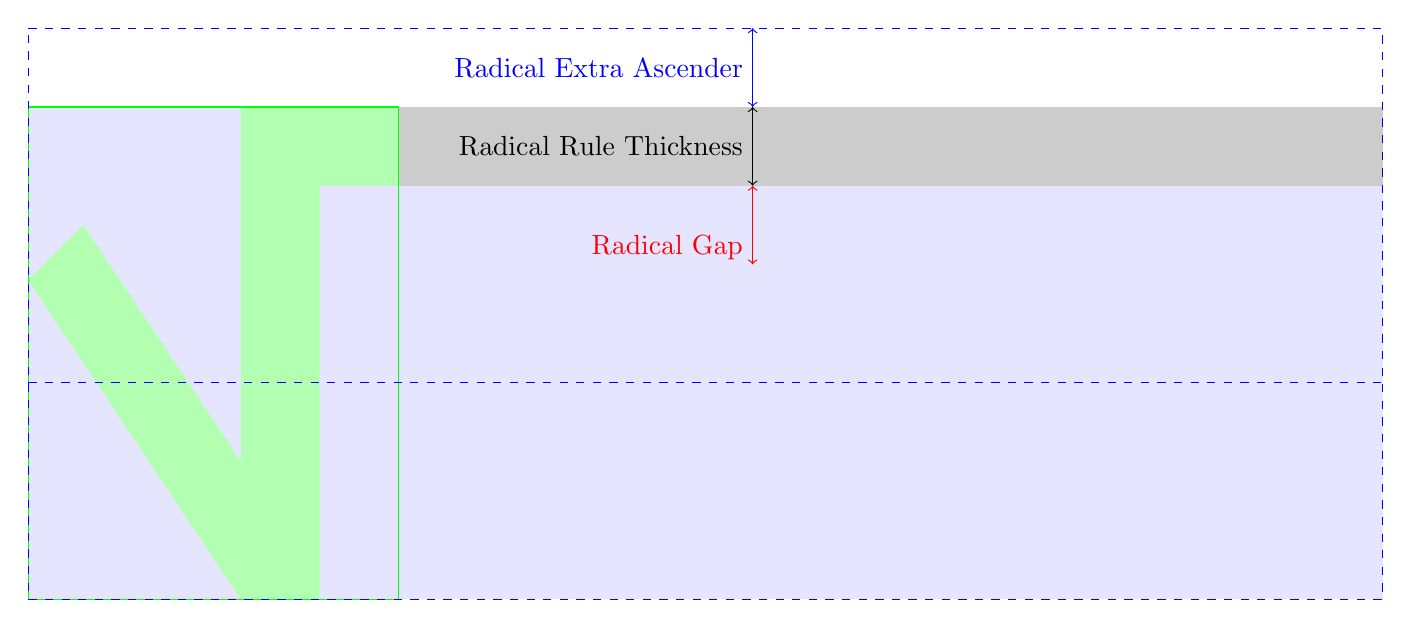
\begin{tikzpicture}[yscale=-1]
  \fill[blue!10] (-4.7,-2.5) -- (12.5,-2.5) --
  (12.5,3.75) -- (-4.7,3.75) -- cycle;

  \fill[black!20] (0,-2.5) -- (12.5,-2.5) -- (12.5,-1.5) -- (0,-1.5) -- cycle;

  \fill[green!30]
  (0,-2.5) -- (-2,-2.5) -- (-2,2) --
  (-4,-1) -- (-4.7,-.3) -- (-2.7,2.7) -- (-2,3.75) -- (-1,3.75) --
  (-1,-1.5) -- (0,-1.5) -- (0,-2.5);
  \draw[green] (-4.7,-2.5) -- (0,-2.5) -- (0,3.75) -- (-4.7,3.75) -- cycle;

  \MathMLBox{0}{1}{2.5}{1}{red}

  \draw[dashed,blue] (-4.7,-3.5) -- (12.5,-3.5) --
                     (12.5,3.75) -- (-4.7,3.75) -- cycle
                      (-4.7,1) -- (12.5,1);

  \draw[<->,blue] (4.5,-3.5) --
  (4.5,-3) node[left]{Radical Extra Ascender} -- (4.5,-2.5);

  \draw[<->,black] (4.5,-2.5) --
  (4.5,-2) node[left]{Radical Rule Thickness} -- (4.5,-1.5);

  \draw[<->,red] (4.5,-1.5) --
  (4.5,-1) node[below left]{Radical Gap} -- (4.5,-.5);
\end{tikzpicture}

\end{document}
